\begin{figure*}[htbp]
 \centering % avoid the use of \begin{center}...\end{center} and use \centering instead (more compact)
 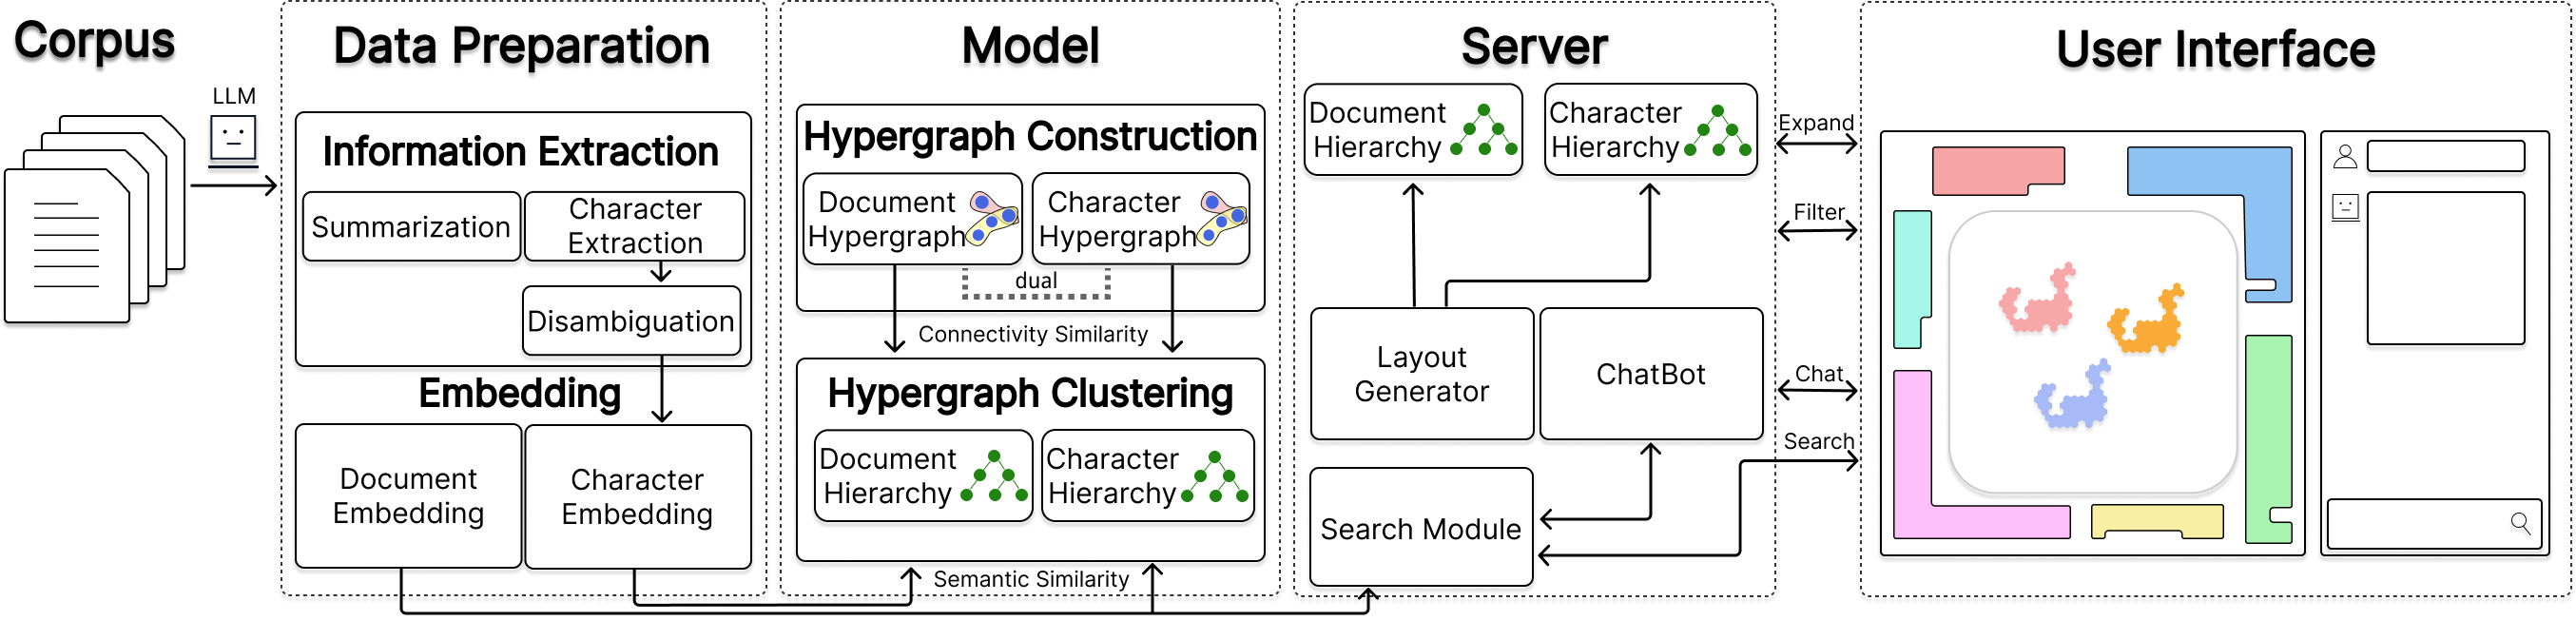
\includegraphics[width=0.95\textwidth]{pipeline}
 \caption{Data processing pipeline of HyperMap. 
 Starting from a corpus of unstructured texts, each document goes through the data preparation stage to extract the main characters.
 Then the documents and characters are both embedded into a vector space.
 The model stage constructs a document hypergraph and a character hypergraph, which are then clustered separately by combining connectivity similarity and semantic similarity.
 The clustered hypergraphs are hosted on the server and visualized in the user interface.
 Users can expand, filter, or search the hypergraphs to explore the corpus and select documents to be analyzed with a chatbot.
  }
\label{fig:pipeline}
\end{figure*}

\section{Design Rationale}~\label{sec: design_rationale}
HyperMap is designed for analysts to explore and reorganize a corpus for their analysis.
Our design rationale to foster interpretation is based on the design guidelines proposed by Chuang et al.~\cite{chuang2012interpretation}.
We reuse their definitions of \textit{Model Alignment}, \textit{Progressive Disclosure}, and \textit{Unit of Analysis} when describing our design rationale.
We first identify common analysis tasks from previous works.
Then, we derive our design considerations (DC) from the analysis tasks.
We take the DCs into account when making our model decisions and visualization design in~\autoref{sec: methodology}.
Finally, we explain how we achieve model alignment by applying the design considerations to our system.

\subsection{Analysis Tasks}
We derive our target analysis tasks from topic- and entity-based approaches.
Topic-based approaches aim to support document understanding by visualizing the topic structure of the documents.
Investigation of the topic structure seeks to answer the question: \textit{What topics are discussed in the corpus, and how are they related?}
Entity-based approaches support investigative analysis by visualizing entities and their relations.
We generalize entities to \textit{Characters}, which are the core entities or concepts discussed in the documents.
For example, in a news article, the characters can be named entities that appear in the title or are involved in the news event.
In a research article, the characters can be the concepts or models proposed by the described work.
Similarly, the investigation of the characters seeks to answer the question: \textit{What characters are discussed in the corpus, and how are they related?}: 
We aim to support both tasks simultaneously as they are fundamental to subsequent tasks and intertwined in a real-world scenario.

\subsection{Design Considerations}
To support the aforementioned analysis tasks, we derive the following design considerations (DCs):
\begin{itemize}
  \item \textbf{DC1: Overview of topic structures and character connections}
  Given a corpus, the topic structures and character connections can be complex and cover a wide range of documents and characters. 
  The overview seeks to cover all the documents and characters by hiding the details.
  This sets the ground for the user to discover their targets of interest.
  \item \textbf{DC2: Progressive Disclosure}
  To facilitate investigation, it is important to support users to drill down from a high-level overview to intermediate abstractions.
  This includes disclosure of a specific topic's sub-structure, the containing documents, and the connections to characters.
  \item \textbf{DC3: Model Alignment}
  Our choice of model should align well with the analyst's mental model when conducting the analysis tasks.
  This means our model should directly operate on the units of analysis, which are topics (groups of similar documents) and characters.
  Then by properly visualizing the abstractions of the model, we are safe to produce a good model alignment.
  \item \textbf{DC4: Detailed analysis of the target of interest}
  The investigation of topic structures and character connections often leads to a target of interest, which can be a topic or a character.
  After such investigation, previous works usually only provide the user with a list of documents that are relevant to the target of interest.
  This is perhaps due to the lack of a unified way to analyze the target of interest under different contexts.
  The advance of LLMs presents a promising solution to this problem by transforming almost any analysis task into a question-answering task.
  We thus include this task to fill the gap in previous works.
\end{itemize}


